%----------------------------------------------------------------------------------------
%	PACKAGES AND DOCUMENT CONFIGURATIONS
%----------------------------------------------------------------------------------------
\documentclass[11pt]{article}
\usepackage{amsmath} % Required for some math elements
\usepackage{hyperref} 
\usepackage{xcolor}
\usepackage{lipsum} 
\usepackage{cite}
\usepackage{graphicx} % Required for the inclusion of images
\usepackage{algorithmic}
\usepackage{array}
\usepackage{bookmark}
\usepackage{listings}
\usepackage{amssymb}
\usepackage{enumitem}
\usepackage{pythonhighlight}
\usepackage[T1]{fontenc}
\usepackage{inconsolata}
\usepackage[margin=8mm]{geometry}
\usepackage[caption=false, font=footnotesize]{subfig}
\usepackage{fancyhdr}
\pagestyle{fancy}
\renewcommand{\headrulewidth}{0.4pt}
\renewcommand{\footrulewidth}{0.4pt}

\usepackage[active,tightpage]{preview}
\renewcommand{\PreviewBorder}{1in}
\newcommand{\Newpage}{\end{preview}\begin{preview}}
  


\newlist{steps}{enumerate}{1}
\setlist[steps, 1]{label = Step \arabic*:}

\hypersetup{ %color attributes of citation, link, etc.
    colorlinks=true,
    linkcolor=blue,
    filecolor=gray,      
    urlcolor=blue,
    citecolor=blue,
}

\newcommand{\matlab}{\textsc{Matlab }} %very important and totally necessary addition
\newcommand{\hdotrule}[1]{\hbox to \textwidth{\leaders\hbox to #1pt{\hss . \hss}\hfil}}

\newcommand\Item[1][]{%
  \ifx\relax#1\relax  \item \else \item[#1] \fi
  \abovedisplayskip=0pt\abovedisplayshortskip=0pt~\vspace*{-\baselineskip}}
%----------------------------------------------------------------------------------------
%	DOCUMENT INFORMATION
%----------------------------------------------------------------------------------------

\title{ECEN 405 \\ Lab 1 PWM Submission}
\author{Daniel Eisen : 300447549}
\date{\today}

\begin{document}
\begin{preview}

      \maketitle
      \hrule
      %----------------------------------------------------------------------------------------
      %	DOCUMENT CONTENT
      %----------------------------------------------------------------------------------------
      \section*{Deliverables}
      \begin{enumerate}
            \item Capacitance:
                  \begin{align*}
                        C_{1} &= \frac{10k}{4{\cdot}8.2k{\cdot}1k{\cdot}30kHz} \\
                              &= 1.016{\times}10^{-8} \\
                        C_{1} &= 10.16nF      
                  \end{align*}
            \item Frequencies: \\
            $R_{1}=8.2k, \; R_{2}=10k, \; , R_{5}=1k, C_{1}=10.16nF$
            \begin{align*}
                        F_{t} &= \frac{(R_{2}+R_{3})}{4R_{1}(R_{4}+R_{5})C_{1}}\\       
                        F_{t}&\{R_{3}=1M ,\; R_{4}=0\} = 3.03MHz \\
                        F_{t}&\{R_{3}=0 ,\; R_{4}=100k\} = 297.1Hz \\
                        \mathrm{to \; match \; lab \; value: \;} F_{t}&\{R_{3}=0 ,\; R_{4}=1M\} = 29.97Hz \\
                  \end{align*}
            \item Schematic:
                  \begin{center}
                        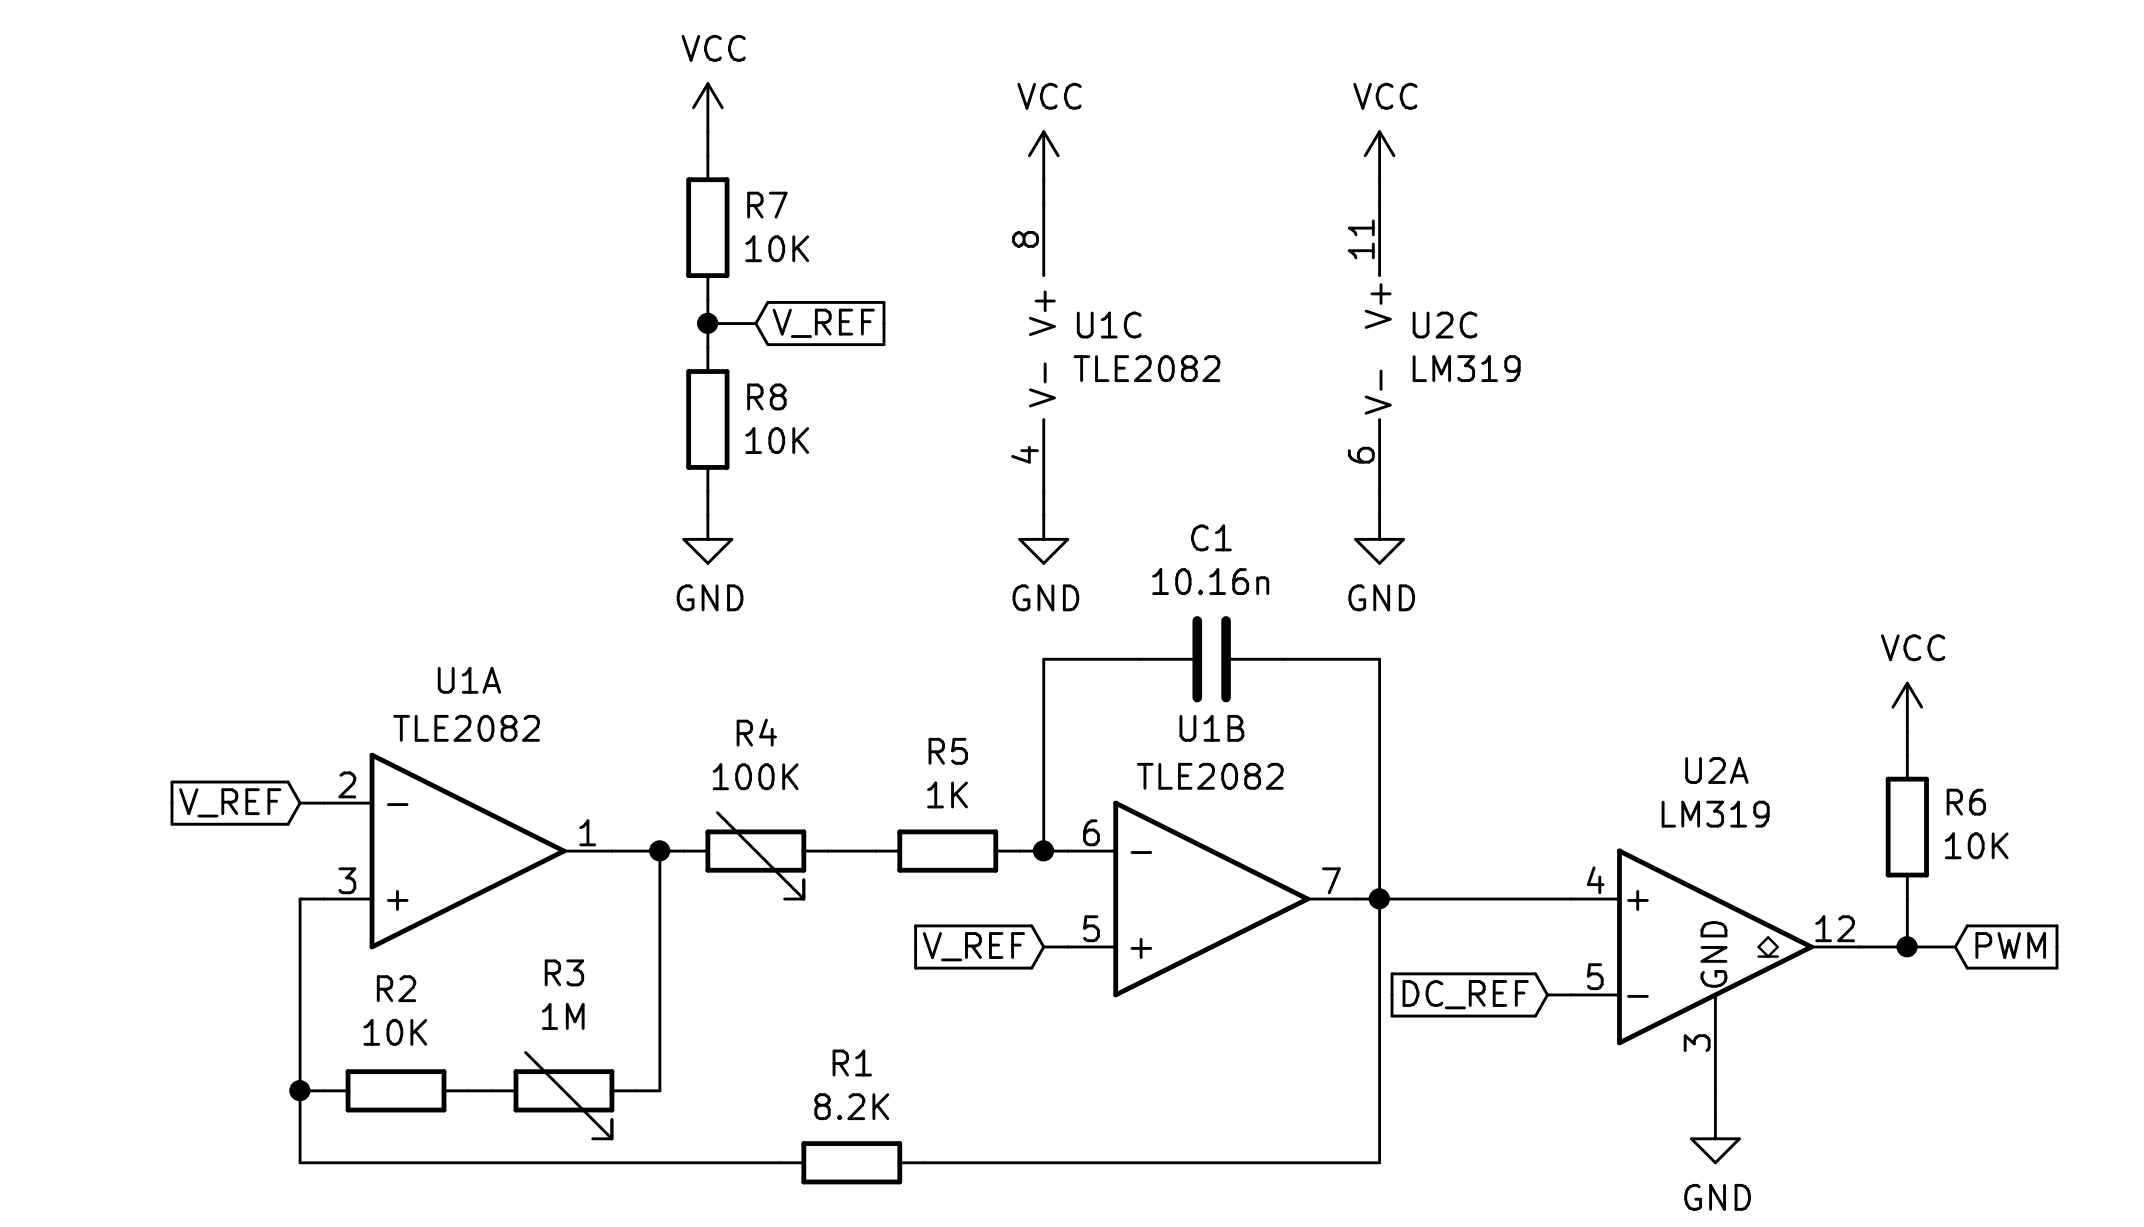
\includegraphics[width=0.75\textwidth]{img/PWM_gen.png}
                  \end{center}
            \item IRFBC40APBF: $R_{DS(on)}=1.2, \; t_{c,on}=13, \; t_{c,off}=31$
                  \begin{align*}
                        \mathrm{Conduction \; losses} = P_{cond} &= R_{DS(on)}dI^{2}\\
                                                                 &= 1.2{\cdot}0.5{\cdot}1\\
                                                                 &= 0.6W \\
                        \mathrm{Switching losses} = P_{sw} &= \frac{1}{2}V_{in}I_{o} \\
                                                      @29.97Hz &= 7.91\mu W \\
                                                      @297.1Hz &= 78.4\mu W \\
                                                      @3.03MHz &= 0.799W
                  \end{align*}
            \item Build it:
                  \begin{center}
                        
\includegraphics[width=0.5\textwidth]{img/thumbs.png} \\
                        \textit{Danny B's approval of breadboarded circuit}
                  \end{center}
            \item Test it:
                  \begin{center}
                        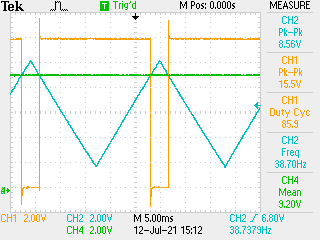
\includegraphics[width=0.3\textwidth]{img/lowest_f.png}
                        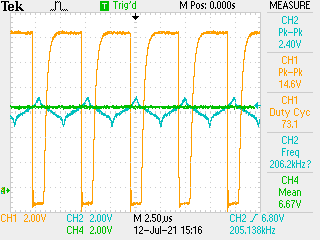
\includegraphics[width=0.3\textwidth]{img/highest_f.png} \\
                        \textit{Lowest Frequency} \hspace*{0.15\textwidth} \textit{Highest Frequency}
                  \end{center}
            \item This circuit is constructed in the real world on a breadboard. So it differs from ideal with parasitic capacitance, imperfect slew rates from the op-amps and comparators and possibly other non-ideal factors. Due to this the upper theoretical frequency (~3Mhz) was could not be achieved, with only a recorded max of ~200kHz.
            \item The LM319 is a duel comparator chip, so to add an inverted output to the circuit the input just need to be switched and fed into the second comparator pins and its out also pulled up. 
            \item This circuit consists of two main subcircuits.
                  \begin{center}
                        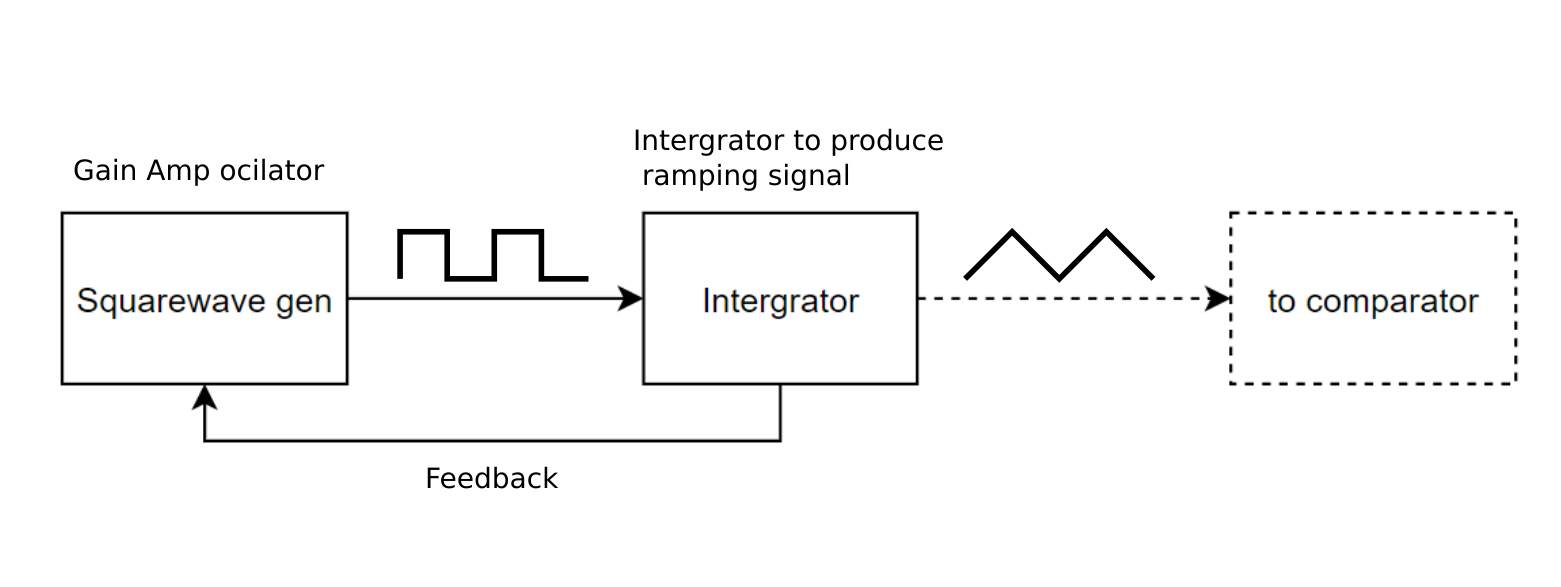
\includegraphics[width=0.75\textwidth]{img/blovk.png} \\
                        \textit{Sub-circuits: Gain Amp Oscillator and Integrator:}
                  \end{center}
      \end{enumerate}
      \hrule
\end{preview}

\end{document}